%This is the first chapter of the dissertation

%The following command starts your chapter. If you want different titles used in your ToC and at the top of the page throughout the chapter, you can specify those values here. Since Columbia doesn't want extra information in the headers and footers, the "Top of Page Title" value won't actually appear.

\chapter[][Recursive Jigsaw Reconstruction]{Recursive Jigsaw Reconstruction}

\textit{Recursive Jigsaw Reconstruction} (RJR) \cite{Jackson:2016mfb,ATLAS-CONF-2016-078} is a novel algorithm used for the analysis presented in this thesis.
RJR is the conceptual successor to the razor technique \cite{Rogan:2010kb,Buckley:2013kua}, which has been used successfully in many new physics searches \cite{SUSY-2014-05,SUSY-2014-06,CMS-SUS-13-004,CMS-SUS-12-005,CMS-SUS-11-024,SUSY-2011-22}.
In this chapter, we will first present the razor technique, and describe razor variables.
We will then present the RJR algorithm.
After the description of the algorithm, we will describe the precise RJR variables used by this thesis and attempt to provide some physical intuition of what they describe.

\section{Razor variables}

In this thesis, we consider SUSY models where gluinos and squarks are pair-produced.
Pair-production is a consequence of the $R$-parity imposed in many SUSY models.
$R-$parity violation is highly constrained by limits on proton decay\todo{CitE}, and is often assumed in SUSY model building.
The Feynmann diagrams considered are shown in Fig.\ref{fig:feynmann_signal}.\todo{Check on W production thing, LO naming}.
\begin{figure}
\caption{Leading order Feynman diagrams for the SUSY signals considered in this thesis} \label{fig:feynmann_signal}
\subfloat[Disquark production]   {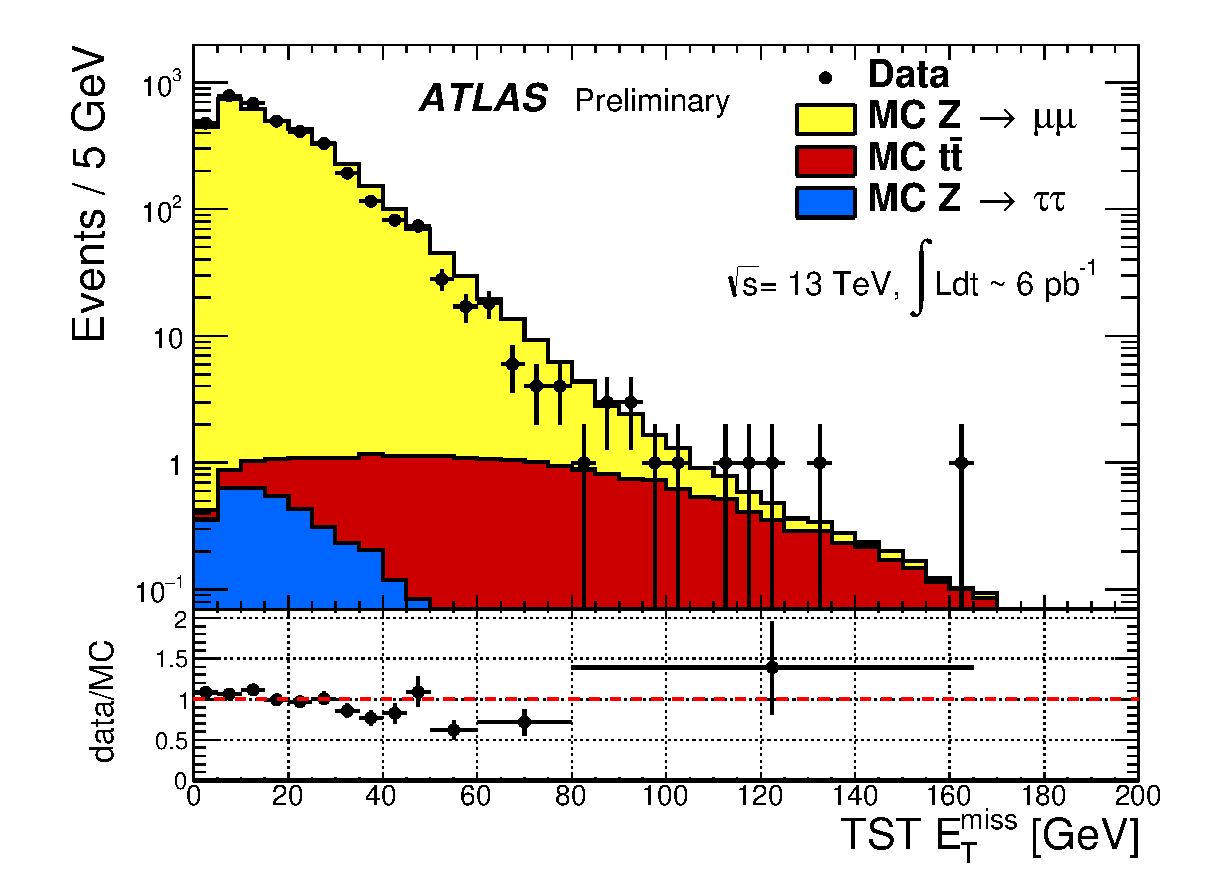
\includegraphics[width=.9\linewidth]{ATLAS-CONF-2016-078/fig_01a}}
\subfloat[Digluino production]   {\includegraphics[width=.9\linewidth]{ATLAS-CONF-2016-078/fig_01b}}
\subfloat[Digluino production with associated W bosons.]   {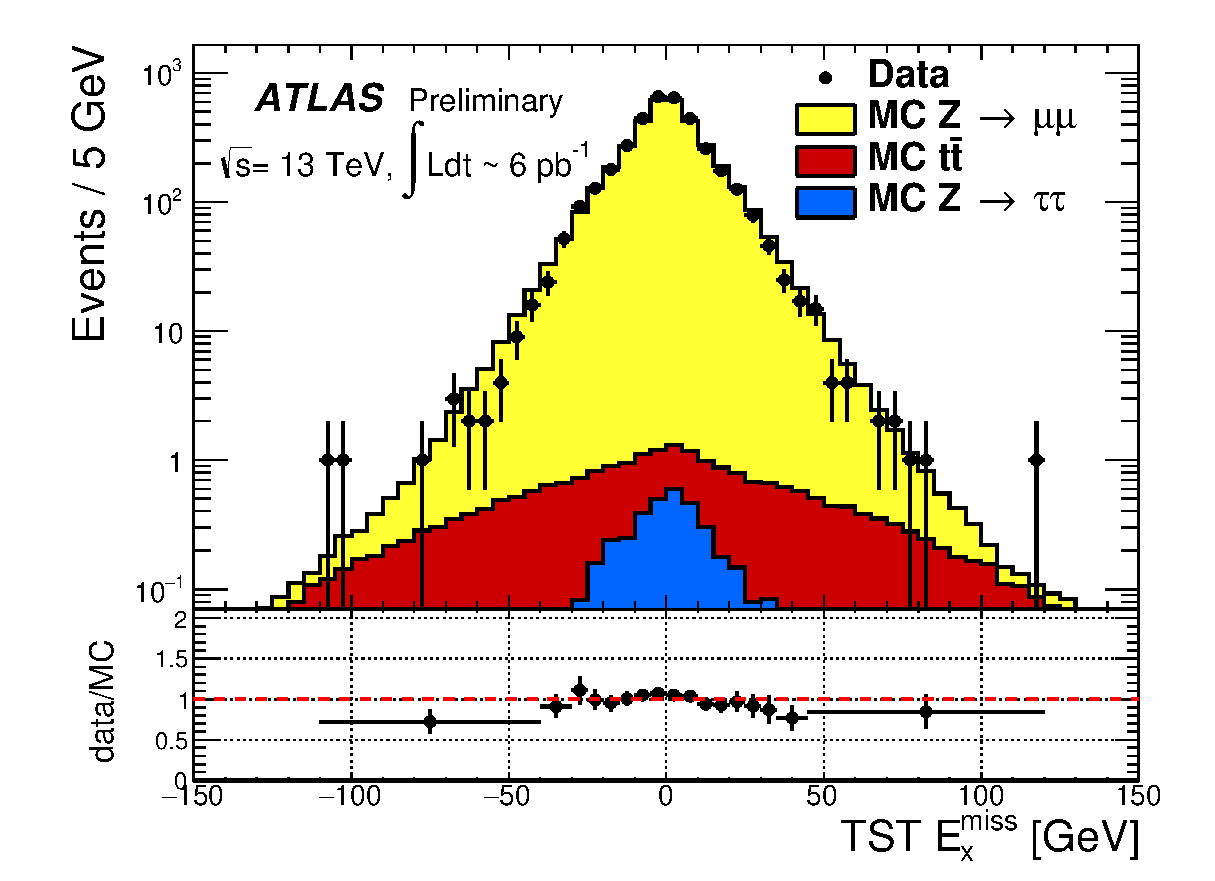
\includegraphics[width=.9\linewidth]{ATLAS-CONF-2016-078/fig_01c}}
\end{figure}

As discussed previously, the consequences of this $\mathbb{Z}_2$ symmetry are drastic.
To understand the utility of the razor variables, the stability of the lightest supersymmetric particle is very important.
The stability of the \textit{lightest supersymmetric particle} is very important.
In many SUSY models, including the ones considered in this thesis, this is the lightest neutralino \lsp.
This means that on either side of a SUSY decay process, where we begin with disparticle production, we have a final state particle which is not detected.
Generically, this leads to \met.
Selections based on \met are very good at reducing dominant backgrounds, for example from QCD backgrounds.

However, there are limitations to searches based on \met.
Due to jet mismeasurements, instrumental failures, finite detector acceptance, nongaussian tails in the detector response, and production of neutrinos inside of jets, there are many sources of ``fake'' \met which does not correspond to a Standard Model neutrino or new physics object such as an LSP.
An additional limitation is the complete lack of longitudinal information.
As events from i.e. QCD backgrounds tend to have higher boosts along the $z$-direction, this is ignoring an important handle in searches for new physics.
Finally, \met is only one object, which is a measurement for \textit{two} separate LSPs.
\todo{say somethign else here}


\subsection{Derivation of the razor variables}

The ``razor'' variables $(M_R, R^2)$ are one of many attempts to alleviate these shortcomings of the \met variable\footnotemark
\footnotetext{The razor variables have undergone confusing notational changes over the years.
We will be self-consistent, but the notation used here may be different from references.
}


\section{Recursive Jigsaw Reconstruction}


The algorithm proceeds by the imposition of a particular \textit{decay tree}, which corresponds to a simplified Feynmann diagram.
At each step in this decay tree, we can calculate variables of interest, through a series of simplifying assumptions.
In order to

\section{Variables used in the search for zero lepton SUSY}